\chapter{提案するシステムの概要}

% TODO: この章でいうこと、言わないことがはっきりしてない。
% Windowing Systemの詳しい話とかはなんのためにするのかわからない。

\section{はじめに}

本章では次章以降の研究課題解決を述べるにあたり,システムの全体像とそれを採用した理由を
既存研究と比較しつつまとめる.

\ref{section:intro:problem}で述べたように,現在の没入環境のパラダイムでは,2次元の
デスクトップ環境とは異なり,基本的に1つのアプリケーションがユーザの環境全体を支配するため,
マルチコンテキストな没入空間は実現できていない.
このため没入環境でも複数のアプリケーションを同時に利用できるようにしようとするのは自然であり,
本論文で提案するシステムでも複数アプリケーションが没入環境で同時に利用できることを
基礎的なシステム要件の1つとする.
ここでの没入環境のアプリケーションとは,ユーザの視野全体を支配するようなものではなく,
机や時計といった空間の一部を占有するようなアプリケーションである.

次節以降ではまず,\ref{section:overview:windowing-system}で2次元のデスクトップ環境での
マルチコンテキストな空間を作り出している重要な技術要素であるWindowing Systemについて,
その特徴をマルチコンテキストという視点からまとめる.
次に\ref{section:overview:related-work}で,関連する研究や他の技術要素について触れ,
最後に\ref{section:overview:conclusion}で本論文の結論として採用したシステムの概要と,
システムが提供する機能のスコープを定義する.

\section{Windowing System}
\label{section:overview:windowing-system}

Windowing Systemとは,2次元のデスクトップ環境で複数のアプリケーションを1つのスクリーン空間で
同時に用いるための仕組みである.さまざまなオペレーティングシステムでの実装があり,
オープンソースな実装としては X.Org\footnote{https://www.x.org/wiki/}による
X Window System\cite{x-window-system}や
Wayland\footnote{https://wayland.freedesktop.org/}などがある.
Windowing Systemは2次元のデスクトップ環境において,ブラウザやメールクライアントなど
複数のアプリケーションを同時に利用することを可能にしているが,アプリケーション間の衝突なく
これを実現するための様々な工夫がある.

まず,Windowing Systemでは,サーバ・クライアントモデルを採用しており,
複数のアプリケーション(クライアント)と,それらとコミュニケーションを行って
ウィンドウをスクリーンに実際に表示するコンポジッタ(サーバ)から構成される.
% 図や、詳しい説明を入れてもいいかも
アプリケーションはそれぞれプロセスとして起動でき,Inter-Process Communication (IPC)に
よってコンポジッタとコミュニケーションをとる.
このためアプリケーションどうしはオペレーティングシステムによってメモリ空間の分割や,
CPUのスケジューリング,セキュリティ上の分離などを行ってもらえ,
基本的なアプリケーションどうしの衝突を防いでいる.
また,2次元のデスクトップ環境では1つのスクリーン空間上に複数のアプリケーションがウィンドウと
呼ばれる長方形領域が重なる形で表示される.
ウィンドウの位置や大きさは基本的にアプリケーション側で決めるのではなく,ユーザが調整できるため,
アプリケーションの空間的な衝突をユーザ自身が最小限にできる.
さらに,ユーザはマウスなどのポインティングデバイスでスクリーン上のカーソルを操作し,
カーソルを介してアプリケーションとのインタラクションを行う.
入力に関するこのプロトコルはカーソルが重なっているウィンドウのみにカーソルのイベントが伝達される
という制約ゆえに,1つのポインティングデバイスの入力イベントを適切にアプリケーションに
割り振っており,ユーザの意図しないアプリケーションが入力を受け取ったり,複数のアプリケーションが
入力を同時に受け取ってしまうといった,入力の衝突を最小限にしている.
Windowing Systemではこういった衝突を防ぐ工夫によって,
それぞれ全く無関係のアプリケーションをどのように組み合わせて用いても,
ある程度使いやすくデスクトップ環境を利用できるようにしている.
マルチコンテキストな空間を実現するためには,市場にある様々なアプリケーションの中から,
ユーザが自由に選んで,その時々のコンテキストに合わせて恣意的にアプリケーションを
組み合わせられる必要があるため,このアプリケーション間の衝突を防ぐ仕組みは,
マルチコンテキストな没入環境を考えるうえでも重要である.

\section{類似研究・技術}
\label{section:overview:related-work}

初めてマルチコンテキストな没入環境を実現するシステムの提案がされたのは
1997年のTsaoらによるCRYSTAL\cite{crystal}である.
CRYSTALはX Windowing Systemに強い影響を受けており,サーバ・クライアントモデルに近い,
MasterSynchronizerとそれぞれ機能を持ったモジュールからなるシステム(図\ref{fig:crystal})
を提案している.ここではモジュールがアプリケーションと近い意味を持つが,
アプリケーションだけではなく,ヘッドトラッキングなど,ハードウェアから提供されるデータも
モジュールとして抽象化されている.単一マシン向けであり,モジュールとMasterSynchronizer
とのコミュニケーションは共有メモリとセマフォを用いた独自のプロトコルで効率的に行っている.
アプリケーションには2次元デスクトップ環境におけるウィンドウのメタファーとして
3D Crystal(図\ref{fig:crystal-window})と呼ばれる直方体領域が割り当てられており,
このようなメタファーは後述するmotorcar\cite{reiling}や
studierstube\cite{studierstube}などでも用いられている.

\begin{figure}[htbp]
  \centering
  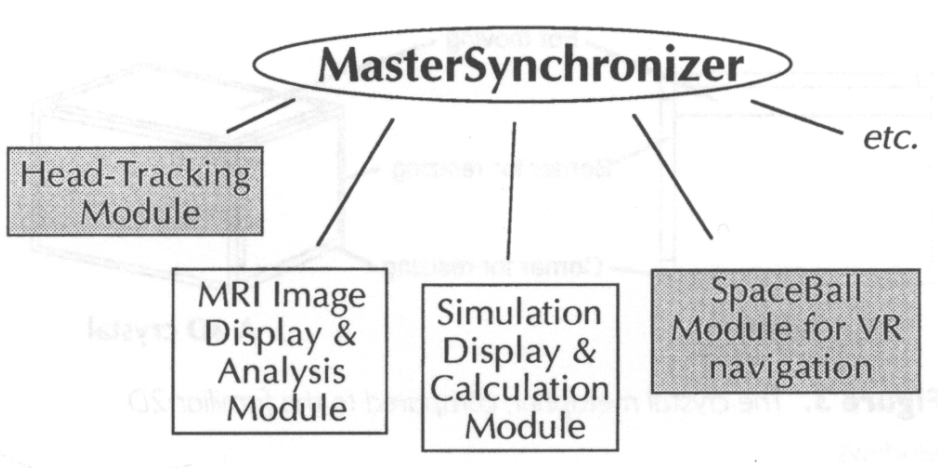
\includegraphics[keepaspectratio, width=0.7\linewidth]{figures/crystal.png}
  \caption{
    CRYSTAL のシステム概要図.MasterSynchronizerとそれぞれ機能を持ったモジュールからなる.
    影のついた箇所はハードウェアコンポーネントである.
    (Adapted from Tsao and Lumsden 1997\cite{crystal})
  }
  \label{fig:crystal}
\end{figure}

\begin{figure}[htbp]
  \begin{minipage}[t]{0.49\linewidth}
    \captionsetup[sub]{margin=0.1cm}
    \centering
    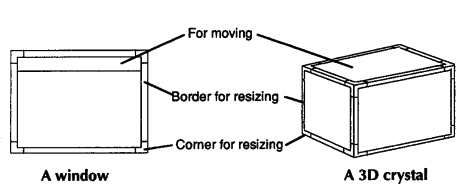
\includegraphics[keepaspectratio, width=\linewidth]{figures/crystal-window.png}
    \subcaption*{}
  \end{minipage}
  \begin{minipage}[t]{0.5\linewidth}
    \captionsetup[sub]{margin=0.1cm}
    \centering
    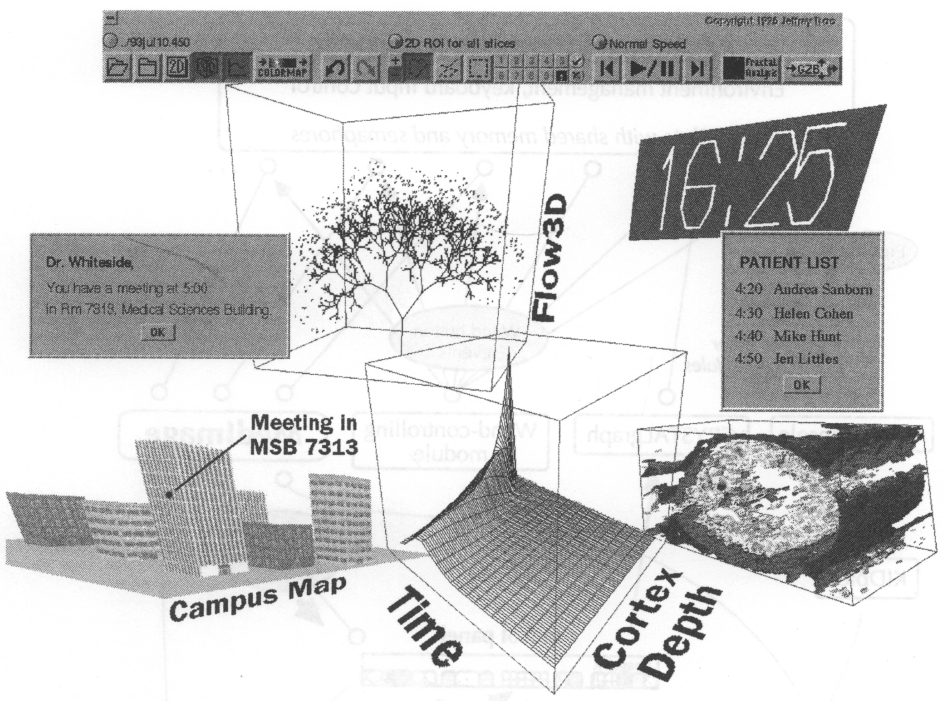
\includegraphics[keepaspectratio, width=\linewidth]{figures/crystal-ve.png}
    \subcaption*{}
  \end{minipage}
  \centering
  \caption{
    CRYSTALで提案された3D crystalの図.左図はウィンドウとのメタファーを説明したもの.
    右図は実際に用いられる状況を想定した図.
    (Both adapted from Tsao and Lumsden 1997\cite{crystal})
  }
  \label{fig:crystal-window}
\end{figure}

SchmalstiegらはARの分野で,複数アプリケーションを表示することに加え,
複数ユーザ・ホストマシンでの利用を想定したシステムである,
Studierstube\cite{studierstube}を提案した.
Studierstubeでは,システムに接続した複数のユーザがアプリケーションの状態や,
現実空間での位置を共有しながら操作する仕組みを提案している.
加えて,同時にアプリケーションの状態は共有しながら,その現実空間の位置はユーザごとに変えることも
可能にすることで,遠隔地からのコラボレーションや,一箇所に集まりきれないほどの大人数での
コラボレーションにも対応できるようなマルチローケルなシステムであることも特徴である.
また,Studierstubeのアプリケーションはプロセスとして起動するのではなく,動的ライブラリとして
システムにロードされ,システムのプロセスの中で呼び出されることも特徴である.

Reilingの提案したmotorcar\cite{reiling}ではLinux上で動くWindowing Systemである
Waylandのプロトコルを拡張する形で3DのWindowing Systemを提案した.
WaylandはLinuxで広く使われていたX Window Systemの,Linuxカーネルやハードウェアの進化と共に
浮き出てきたパフォーマンス上の欠点などを解消する形で生まれたWindowing Systemである.
基本的な2次元のWindowing Systemを構成するのに必要なプロトコルが定義されているのに加え,
自由にプロトコルを拡張できる仕様になっており,motorcarでは,拡張したプロトコルに沿って
コンポジッタがアプリケーションから3Dオブジェクトを表示するための情報を受け取り,
複数のアプリケーションから受け取った情報を合成して,ヘッドマウントディスプレイ(HMD)に
出力している.
既存の2次元デスクトップのWindowing Systemの拡張であるため,Studierstubeとは違い,
シングルホストマシンにおいて複数の3Dアプリケーションを利用できるシステムであるが,
既存の2DWaylandアプリケーションからのデータも同様に受け取ることができ,
それを没入環境に3Dアプリケーションと同時に表示できる.

近年の産業的な成果に目を向けても,マルチコンテキストに対応しようとする動きがみえる.
特に既存の2Dのアプリケーションを没入環境に表示することで,
没入環境のマルチコンテキスト化を図る例は多い.
2次元のPCの画面を没入空間で使えるようにするものとしては,
Virtual Desktop
\footnote{Virtual Desktop. Inc. ``Virtual Desktop'' https://www.vrdesktop.net/ (accessed 25 Dec, 2022)}
のような専用のVRアプリケーションや,
Meta Horizon Workrooms
\footnote{Meta. ``Meta Horizon Workrooms'' https://www.meta.com/jp/work/workrooms/ (accessed 25 Dec, 2022)}
やSpatial
\footnote{Spatial Systems, Inc. ``Spatial'' https://www.spatial.io/ (accessed 25 Dec, 2022)}
といった会議やイベント用のVRアプリケーションの中でPC画面を投影するものなどがある.
また,Microsoftの提供するMixed Reality HMDであるHoloLens
\footnote{Microsoft ``HoloLens'' https://www.microsoft.com/ja-jp/hololens (accessed 25 Dec, 2022)}
や Meta社の提供するMeta Quest
\footnote{Meta ``Meta Quest'' https://www.meta.com/jp/quest/ (accessed 25 Dec, 2022)}
では特定の形式の2Dアプリケーションを没入環境で複数起動できる仕組みがある.
ただし,これらは没入環境自体をマルチコンテキスト化しているわけではなく,
没入環境にマルチコンテキストな2Dデスクトップ環境を持ち込んでいると捉えられる.

さらに,VRやARのシステムの標準化におけるデファクトスタンダードであるOpenXR
\footnote{Khronos group ``OpenXR'' https://www.khronos.org/openxr/ (accessed 25 Dec, 2022)}
では.Overlayと呼ばれる機能が定義されており,メインのユーザの視野全体を支配する
アプリケーションに重ねて,他のコンテンツを表示できる仕組みを提供しており,
VRゲームをプレイしながら,ソーシャルメディアを時々チェックするといった,
マルチコンテキストな没入環境の使い方を支援している.

\section{本論文での結論}
\label{section:overview:conclusion}

本論文での結論としては,Waylandのプロトコル拡張の機能を用いる Reiling の手法を基本的な
システム構成のベースとした(図\ref{fig:overview}).
システムの構成要素は,3DアプリケーションとWayland上で動作する既存の2Dアプリケーション,
入力装置であるキーボードとマウス,没入環境を提示するHMD,そしてそれらとコミュニケーションを
とって制御する3Dコンポジッタである.
3Dコンポジッタはマウスやキーボードの入力を適切にアプリケーションに分配し,
2D/3Dアプリケーションは没入環境に描画したい内容を3Dコンポジッタに伝える.
3Dコンポジッタは複数のアプリケーションから受け取った情報を合成してHMDに表示することで,
ユーザに複数アプリケーションが利用可能な没入環境を提示できる.

% TODO: 入力に関してはFuture workであることをここで述べるのもあり.

本論文が扱うのは3Dアプリケーションとコンポジッタとの間のやり取りのプロトコル,
また3Dコンポジッタの設計・実装の部分である.
2Dアプリケーションとコンポジッタとの間のプロトコルは既存のものが存在しており,
本論文のスコープの範囲ではないが,他の部分の設計において重要な要素であり,
詳しくは\ref{chapter:2d}章で扱う.

\begin{figure}[htbp]
  \centering
  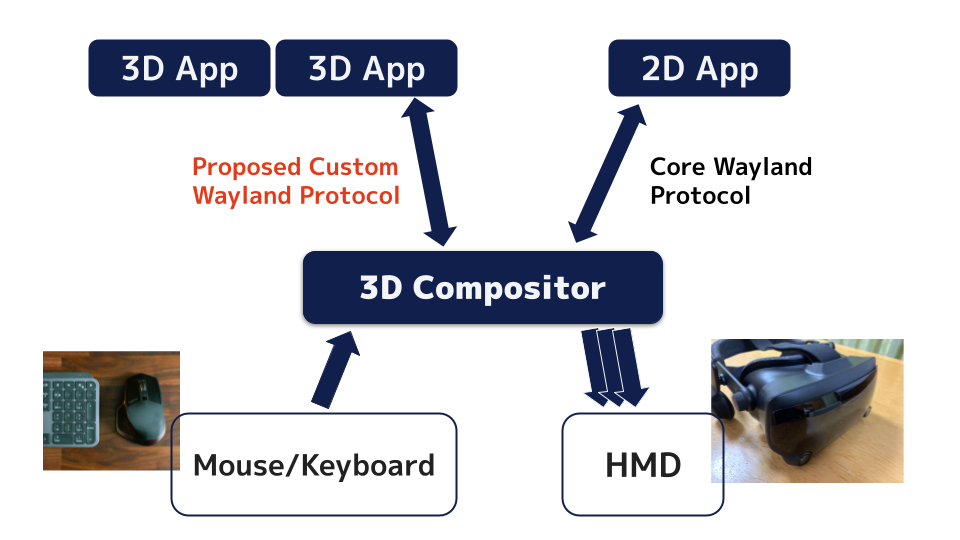
\includegraphics[keepaspectratio, width=\linewidth]{figures/overview.png}
  \caption{提案するシステムの概要図.}
  \label{fig:overview}
\end{figure}

類似研究・技術と比較してこの設計を選択した理由は以下の通りである.
\begin{itemize}
  \item マルチコンテキストな没入環境を社会実装していくうえで大きな課題となるのは,
        初期の3Dアプリケーションの少なさである.
        ユーザの視野全体を覆うというパラダイムのアプリケーションから,空間の一部を占有する
        アプリケーションへと変えようとしているため,既存の3Dアプリケーションを少し改変して
        対応できるわけではない.
        しかし豊富に存在する既存の2Dアプリケーションが,没入環境で使うことができれば,
        3Dアプリケーションは,例えば3Dモデルをみるだけといった,補助的な役割から
        始めることができる.
        このため既存の2Dアプリケーションを利用できるようにすることは大変重要であると考える.
        CRYSTALやStudierstube,OpenXRのOverlayなどは2Dアプリケーションを表示する
        仕組みとは全く異なる仕組みを用いているため,既存の2Dアプリケーションを
        利用することは不可能,または制限がかかることになる.
        一方,本論文が採用したシステムでは,2Dアプリケーションと直接やり取りするコンポジッタを
        自由に設計し直せるため,没入環境で2Dアプリケーションを最大限利用できる.
        その詳細は\ref{chapter:2d}章で述べる.

  \item 本システムは単一ホストマシンでの利用のみをスコープとしており,Studierstubeのような
        複数のホストマシンでの多人数の利用に関してはスコープに入れていない.
        どのように多人数でのコラボレーションを実現するかは,自明でないためである.
        例えば,ユーザの間で同期されるべきデータについても,3Dモデルを共同編集するような
        アプリケーションであれば,メッシュやテクスチャのデータを同期しなければいけないが,
        同時にある動画を見るアプリケーションであれば,同期するべきデータは動画のIDと再生時間
        のみで良い可能性がある.その他にも同期の頻度やタイミング,操作や閲覧の
        権限管理をするかなどは個別のアプリケーションによって替わりうる.
        また,サーバなどインフラやその他の機器を必要とする場合もありえる.
        このため個別の3Dアプリケーションがサーバなどを介して,
        サービスとして多人数コラボレーションを実現するのが現実的だと考えられる.

  \item \ref{section:background}で述べたように,没入環境を用いた3Dアプリケーションは
        様々な分野で応用されており,単に没入環境にPCの画面を投影するだけでは
        没入環境を最大限利用できていない.
\end{itemize}

% Windowing Systemを利用すること。
% マルチコンピュータでの相互互助などはそれぞれのClient Applicationに任せる方針を取る。
% それ以外にもすること、しないことをはっきりさせたい。
